\documentclass[a4paper]{article}

\usepackage[english]{babel}
\usepackage[utf8]{inputenc}
\usepackage{amsmath}
\usepackage{graphicx}
\usepackage{listings}
\usepackage[colorinlistoftodos]{todonotes}
\title{Emergent Architecture Design}
\usepackage{authblk}

\author[1]{Boudewijn van Groos}
\author[2]{Chris Langhout}
\author[3]{Jens Langerak}
\author[4]{Paul van Wijk}
\author[5]{Louis Gosschalk}

\affil[1]{bvangroos \\
4229843}
\affil[2]{clanghout \\
4281705}
\affil[3]{jlangerak \\
4317327}
\affil[4]{pjvanwijk \\
4285034}
\affil[5]{lgosschalk \\
4214528}

\date{\today}

\begin{document}
\maketitle
\tableofcontents
\newpage

\section{Introduction}
\subsection{Design goals}
 	\begin{itemize}
    \item Modularity:
    The program can be split into a number of modules. These modules should be implemented independently of the other modules. Interaction between modules is only possible by making use of defined interfaces.
    \item Continues Integration: There should be always a working product. Each sprint should add one or more feathers. 
		\end{itemize}

\section{Software architecture views}
\subsection{Subsystem decomposition}

\begin{figure}[h]
	\centering
   	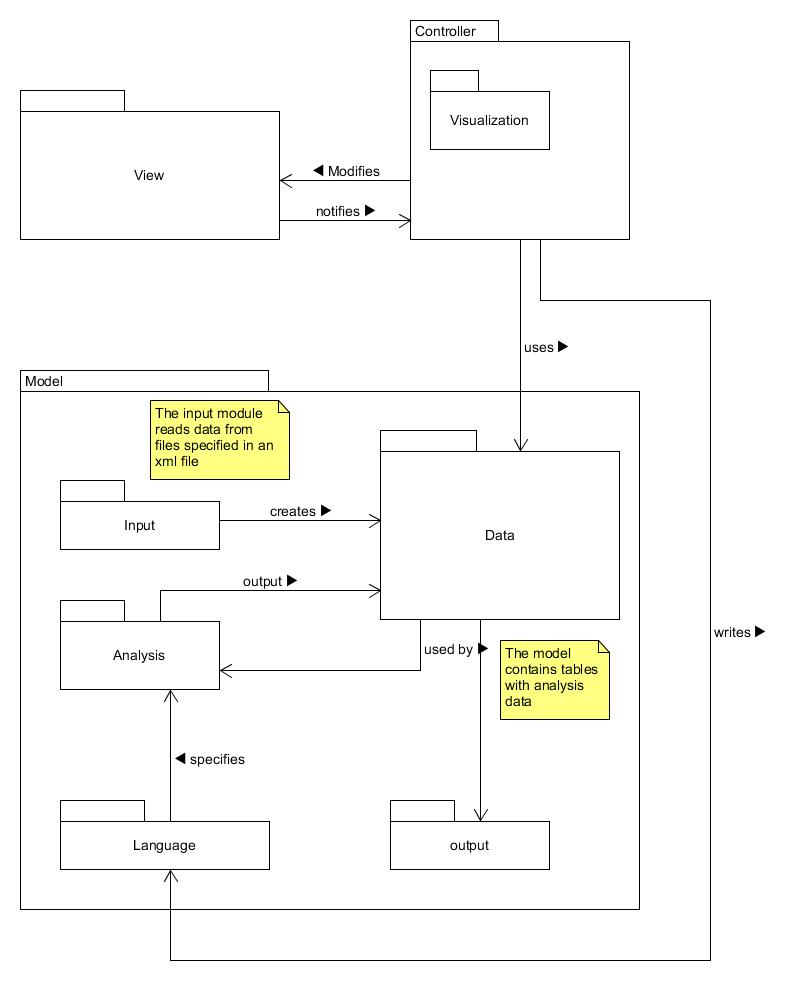
\includegraphics[scale=0.6]{images/modules.jpg}
    \caption{Modules of the system}
    \label{fig:modules}
\end{figure}
The input module should be able to read the data. With that data a dataModel can be constructed. \\
The Analysis Specification module processes the script that defines how the data should be analyzed. The user provides this script. This module translate the script in operations that can be performed by the Analysis Module.\\
The Analysis Module perform the analyses over the dataModel. The output of this module is the result of the analysis, this is a dataModel.\\
The Visualization module creates a certain visual representation of a dataModel. For example it can create a box-plot of the creatine levels.


\section{Software architecture}

\subsection{Programming languages and programs}

\subsection{Used librarians}


\section{Design goals}

\subsection{Availability}

\subsection{Manageability}

\subsection{Performance}

\subsection{Reliability}

\subsection{Scalability}

\subsection{Securability}


\section{Code quality}


\section{Functional Tests}

\subsection{Unit testing}

\subsection{Integration testing}


\section{Non-functional Tests}

\subsection{Functionality}

\subsection{Usability}

\subsection{Reliability}


\section{Glossarium}

\end{document}
